% Two different strands here - Disease biology (the problem) 
% and sequencing technology (the method) to generate insight

\chapter{Introduction}

\section{Amyotrophic Lateral Sclerosis and Frontotemporal Dementia comprise a spectrum of disease} % the disease problem

%introduce two diseases, compare and contrast
Amyotrophic Lateral Sclerosis (ALS) is a progressive neurodegenerative disorder primarily affecting the motor neurons of the cerebral cortex and the spinal cord. It affects between 2 and 16 people per 100,000 \citep{Logroscino2010}. 
Patients gradually lose voluntary motor control of their limbs and the muscles involved in speech and swallowing. 
Death usually occurs within 2-3 years after the first sign of symptoms, usually from infection caused by the inability to swallow. 
Frontotemporal Dementia (FTD) is a progressive neurodegenerative disorder primarily affecting the frontal and temporal lobes of the cerebral cortex. 
It affects 15-22 people per 100,000 and is the second most common dementia after Alzheimer's disease \citep{Onyike2013}. 
Depending on the subtype of FTD, patients exhibit worsening behavioural inhibition, language production or comprehension. 
Both disorders peak in incidence at around 60 years of age, are invariably fatal and have no cure. 
These two disorders are now recognised to be two ends of a spectrum of disease called ALS/FTD. 
This is in part due to a sharing of symptoms in some cases, as FTD patients can exhibit motor deficits and ALS patients can exhibit cognitive decline, but also due to a striking concordance in pathology and genetics.  % ref

Both disorders have recognisable brain pathology upon autopsy, with the affected brain regions showing aggregated protein inclusions in the nucleus and cytoplasm of neurons and glia. In FTD around 35\% of patients have inclusions that contain Tau, a microtubule-associated protein also linked to Parkinson's and Alzheimer's disease \citep{Rademakers2004}. 
The rest of FTD patients present inclusions containing one of two proteins: TAR DNA-binding protein 43kDa (TDP-43) \citep{Neumann2006, Arai2006} or fused in sarcoma (FUS) \citep{Neumann2009}. In ALS almost all patients present with TDP-43 positive inclusions \citep{Neumann2006, Arai2006} and a small number display FUS inclusions \citep{Vance2009-ye,Kwiatkowski2009}, firmly cementing the link between the two disorders and a suggesting key role for TDP-43 and FUS in ALS/FTD.

% Genetics - following SOD1, the identification of rare TARDBP and FUS mutations.  
The progress in understanding the pathology of ALS/FTD has been mirrored by the progress in locating causative genes. 
This was initially done by linkage studies, where blocks of shared genetic variation were identified in the affected members of large families. 
\textit{SOD1} was the first gene linked to ALS in series of families over 20 years ago \citep{Rosen1993}. 
Patients with SOD1 mutations have SOD1 containing inclusions and not TDP-43.
Mutations in \textit{MAPT}, the gene coding for the Tau protein were then found in familial FTD cases \citep{Hutton1998}, linking the protein pathology with alterations to the gene itself. 
This theme continued in the discovery a series of rare mutations in \textit{TARDBP}, the gene that codes for TDP-43 in familial cohorts of ALS, FTD and combined ALS/FTD \citep{Sreedharan2008-xv, Kabashi2008, Benajiba2009,Borroni2009}. 
Mutations in FUS were then found in ALS patients \citep{Vance2009-ye, Kwiatkowski2009}, completing the link between pathology and genetics.
Shortly after this, a long-standing mystery was solved.
Multiple ALS and FTD families had been linked to a region on chromosome 9, which was revealed to be a large expansion in the intron of the \textit{C9orf72} gene \citep{Renton2011,DeJesus-Hernandez2011}. 
In individuals of Caucasian ancestry the expansion is found in 5-10\% of sporadic ALS and FTD cases, 40\% of ALS and 25\% of FTD cases with a family history \citep{Majounie2012}, more than all the other known genes put together, making \textit{C9orf72} the single largest genetic contribution to ALS and a major contributor to FTD. 
Patients with \textit{C9orf72} expansions have TDP-43 pathology, as well as RNA foci containing the expanded \textit{C9orf72} RNA and dipeptide repeat proteins which are translated from the \textit{C9orf72} repeat sequence in both sense and antisense direction \citep{DeJesus-Hernandez2011, Renton2011}. %UPDATE REFERENCES FOR DPRS and FOCI

The emergence of next-generation sequencing technologies has moved the gene hunting field from conducting linkage in family pedigrees to large-scale studies comparing the allele frequencies between groups of affected and unaffected people, at first in exomes (the total protein coding portion of the genome) and now to whole genomes. 
These studies have found extremely rare mutations that individually account for a very small number of cases but provide vital information on which cellular pathways are involved in disease  \citep{Taylor2016,Pottier2016}.
Broadly, the proteins these genes code for can be grouped by their functions into three categories. 
\textit{OPTN} \citep{Maruyama2010} , \textit{UBQLN2} \citep{Deng2011}, \textit{SQSTM1} \citep{Fecto2011}, \textit{CHMP2B} \citep{Skibinski2005} and \textit{TBK1} \citep{Cirulli2015,Freischmidt2015} have all been linked to protein degradation. 
\textit{MAPT}, \textit{DCTN1} \citep{Puls2003} , \textit{CHCHD10} \citep{Bannwarth2014} and \textit{TUBA4A} \citep{Smith2014} have been linked to microtubule transport and stability. 
The third group of genes encode RNA-binding proteins, and this is the function of \textit{TARDBP} and \textit{FUS}. 
Other RNA-binding proteins associated with ALS/FTD through genetics are \textit{ATXN2} \citep{Elden2010}, \textit{TAF15} \citep{Ticozzi2011}, \textit{hnRNPA1} and \textit{hnRNPA2B1} \citep{Kim2013}, \textit{MATR3} \citep{Johnson2014}, \textit{SFPQ} \citep{Thomas-Jinu2017}, and \textit{TIA1} \citep{Mackenzie2017}. 
The proteins these genes code for have been linked to splicing, transcription, translation and transport of mRNA. 
The converging evidence from the pathology and genetics together create the RNA hypothesis of ALS/FTD, where impaired RNA regulation due to mutations or mislocalisation of RNA binding proteins is progressively toxic to neurons. 
Understanding and refining this hypothesis is the focus of my PhD, although the other genetic results suggest it is only one facet of a complex set of disease pathways. 

\section{RNA splicing is a key step for RNA regulation}

\begin{figure}[h!]
	\centering
	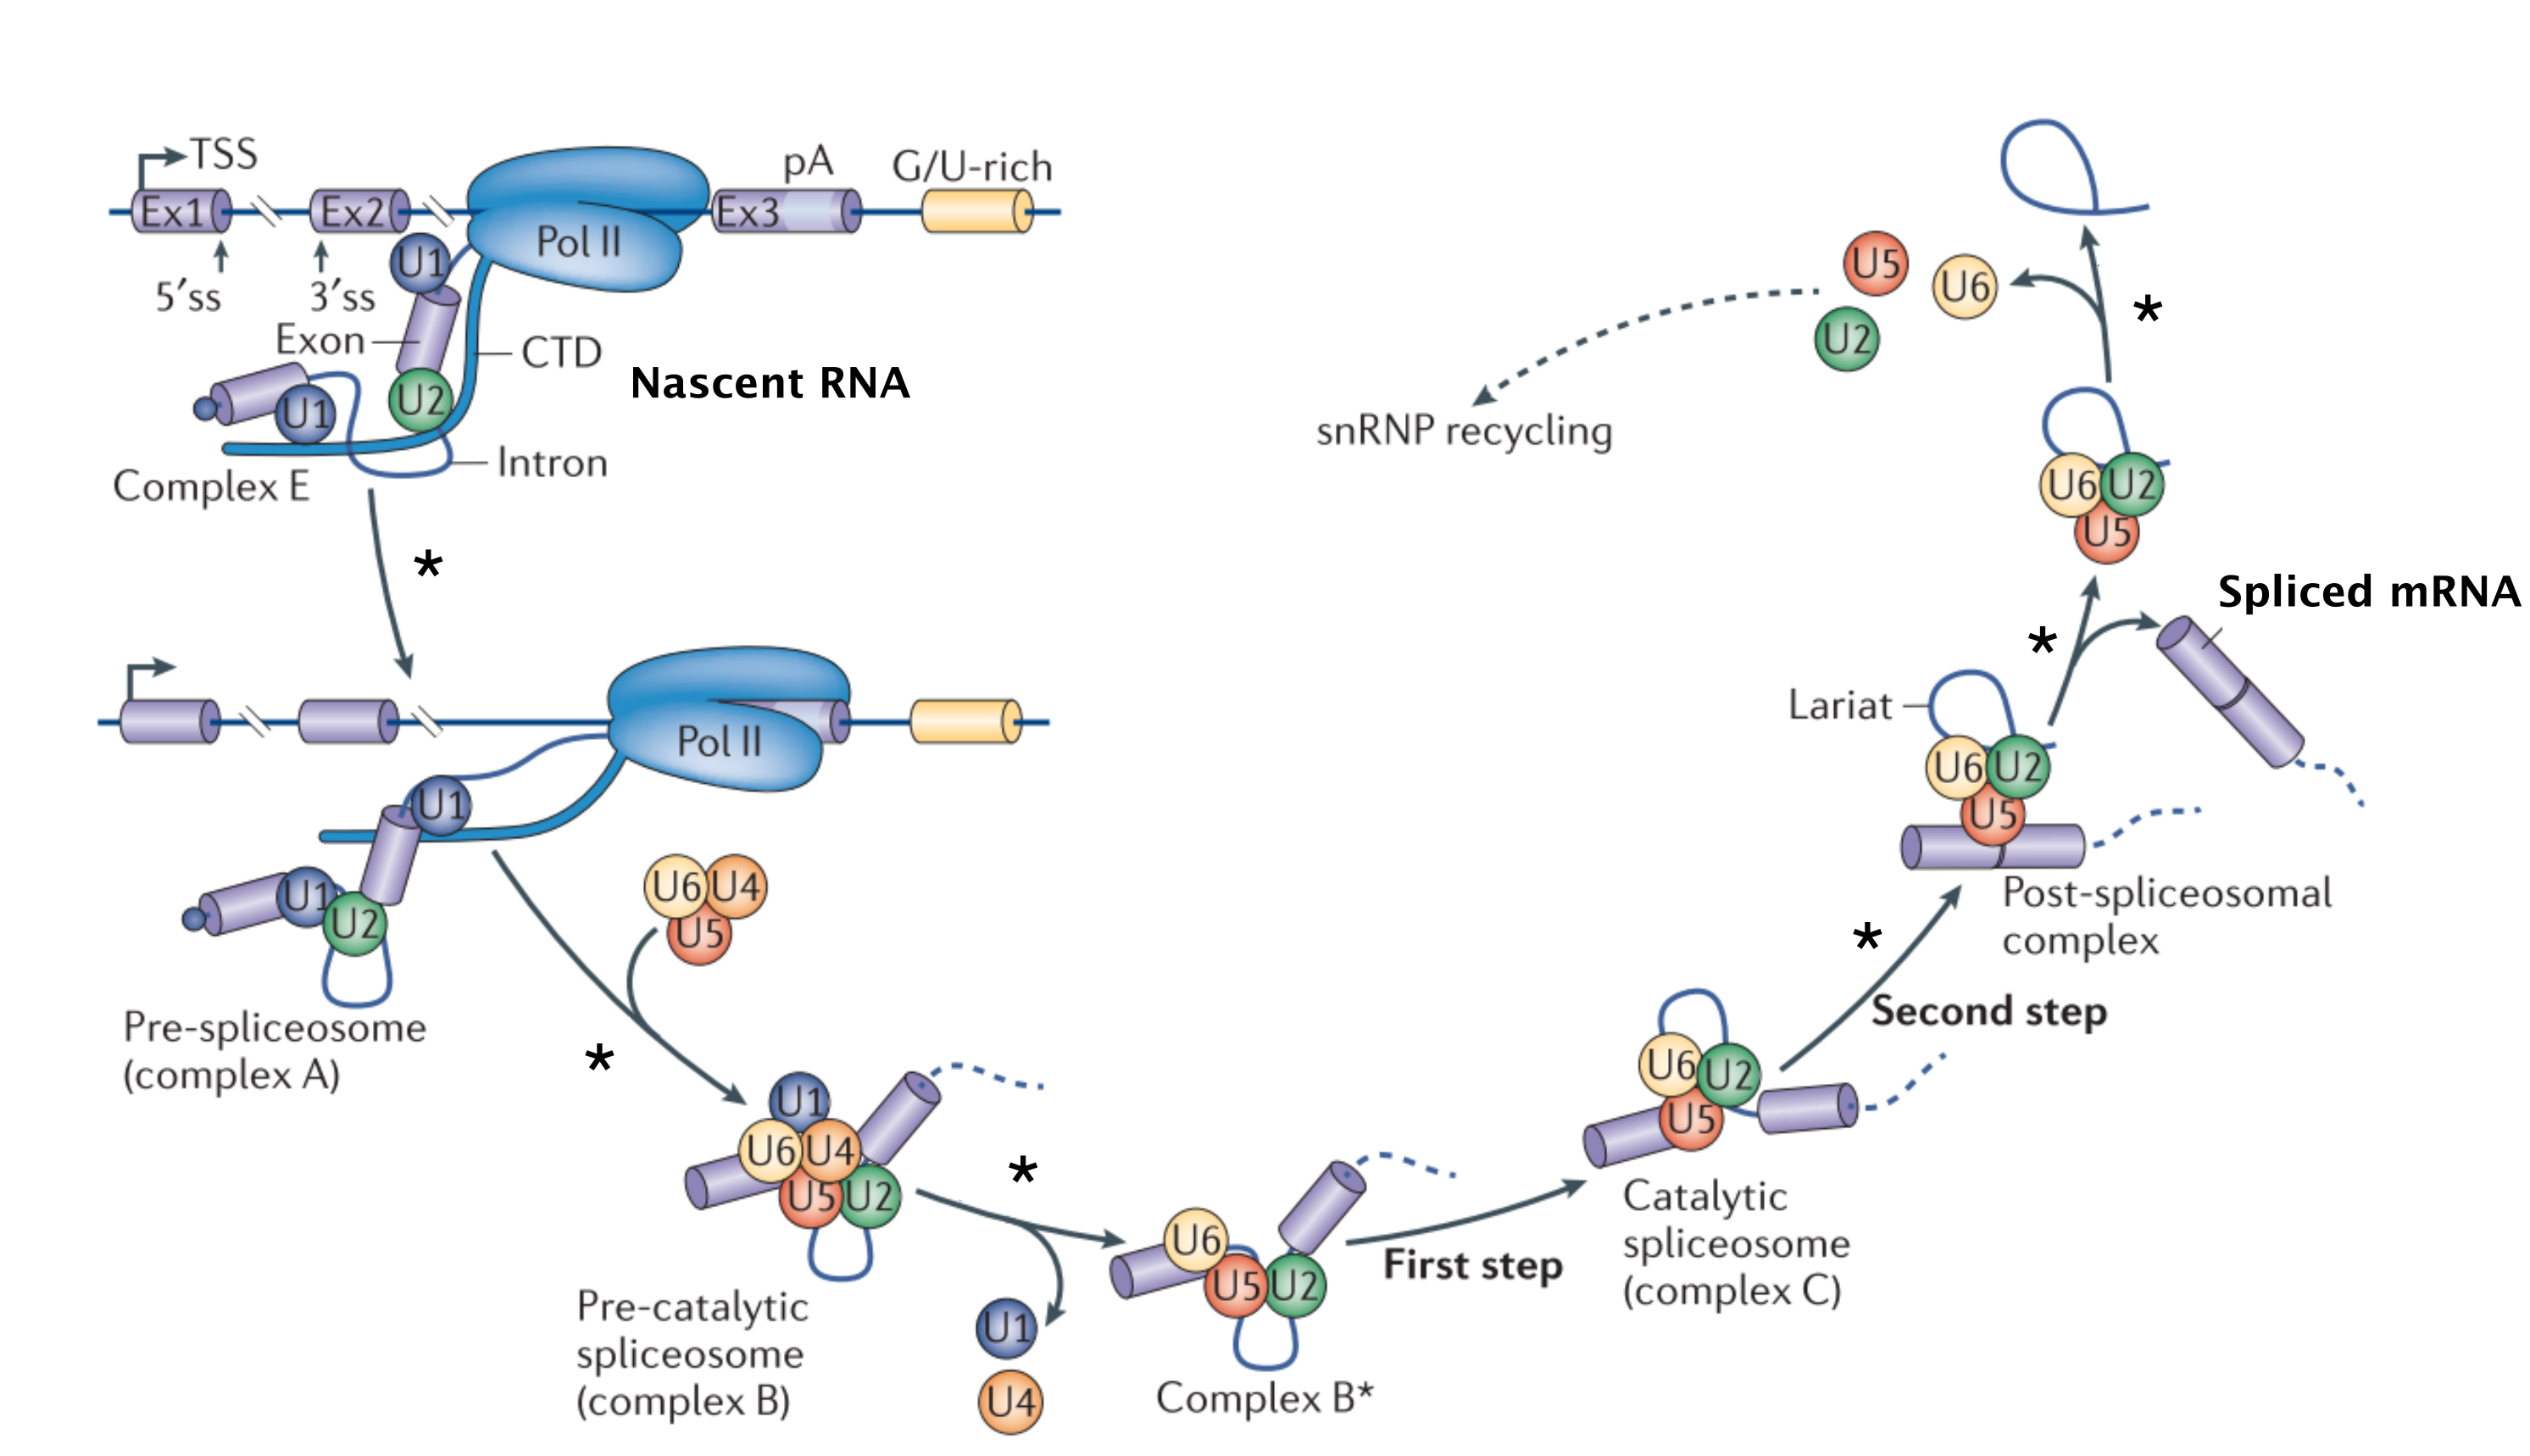
\includegraphics[width=\textwidth]{Figures/01_introduction/splicing.png}
	\caption[Splicing of a U2-dependent intron]{
		\textbf{Splicing of a U2-dependent intron.}
		Splicing proceeds through the recruitment of snRNP particles on the nascent RNA and the formation of different complexes, which transition through different arrangements. 
		* denotes the transition is dependent on the action of ATP and RNA helicases to proceed.
		Figure taken from \citep{Matera2014}. Names of specific helicases have been removed for simplicity.
	 }
	\label{fig:intro_splicing}
\end{figure}

The discovery of a large discrepancy between the length of a gene and the length of its mRNA ushered in new paradigm for biology: RNA splicing \citep{Berget1977,Chow1977}.
This is in essence a process of distinguishing which sections of a nascent RNA molecule are to be kept (the exons), and which are to be removed (the introns) to create a final transcript.
The majority of protein-coding genes are made up of multiple exons and so require splicing for the creation of their mature mRNAs. 
Beyond this, 95\% of multi-exon genes are alternatively spliced \citep{Pan2008,Wang2008}. 
Alternative splicing is the process where a particular set of exons in a gene are selected to be spliced together.
For protein-coding genes this is a mechanism for creating functional diversity in the proteome, where a single gene can encode multiple proteins with different functions.
This has consequences for understanding gene regulation and cell biology.

Splicing depends on the reliable recognition of exons and subsequent removal of introns by the spliceosome complex. 
The spliceosome is a dynamic molecular machine made up of small nuclear ribonucleoprotein (snRNP) complexes containing small nuclear RNAs (snRNA) and their partnering proteins \citep{Matera2014}. 
Splicing proceeds by a set of interactions between the nascent RNA and the snRNP complexes (Fig. \ref{fig:intro_splicing}).
Eukaryotes have two types of introns which are spliced by separate groups of snRNPs: major or U2-dependent introns, and minor or U12-dependent introns. 
Major introns make up 99.5\% of human introns. I will describe the process of U2-dependent intron splicing.

snRNAs form base-pairing interactions with consensus RNA sequences called splice sites. 
These demarcate the boundaries between introns and exons. 
The 5\'\ splice site is recognised by the U1 snRNP and the 3\'\ splice site and the upstream branch point sequence is recognised by the U2 snRNP.
U1 snRNP binding precedes the U2 snRNP and the two complexes first pair together across an exon in a process known as exon definition. 
This is due to the long length of introns in higher eukaryotes that immediate pairing across the intron is unfavoured.
This complex transitions to an intron-defined arrangement across the adjacent intron which brings the two splice sites and the branch point into close contact.
At this point the U4/5/6 tri-snRNP is recruited and through a set of ATP-dependent rearrangements the spliceosome catalyses two transesterification reactions to remove the intron and join the two exons together.
The intron is circularised at the branchpoint to form a lariat structure which is then degraded.

% RBPs and alternate splicing
During splicing, other sequences in the nascent RNA can recruit RNA-binding proteins to modulate splicing by promoting or repressing the splicing of particular exons.
This is the mechanism behind alternative splicing and is an interplay between the \textit{cis}-acting RNA sequence and \textit{trans}-acting proteins.
Whether an exon is included in a mature mRNA transcript depends on the local environment around the splicing reaction.
Sequence motifs can be classified based on which factors they recruit and by what the result of binding is, whether binding enhances or silences the splicing of the exon.
Therefore a motif in an exon that promotes its inclusion is an exonic splicing enhancer element. 
Whether a sequence is used to silence or enhance the splicing of an exon depends on its location within the exon-intron structure.
For example, the neuro-oncological ventral antigen (NOVA) proteins have a binding preference for YCAY sequences, where Y indicates a pyrimidine \citep{Buckanovich1996,Jensen2000}.
NOVA binding directly immediately downstream or distally upstream of an exon acts to promote its inclusion, whereas binding directly on top of an exon or adjacent to the upstream exon promotes exon skipping \citep{Ule2006}.
Multiple splicing factors can bind the same sequence elements and function as a network depending on their levels of expression \citep{Wang2013a}.
These splicing networks can be created by protein-protein interactions between factors or through protein-RNA interactions whereby a splicing factor can control its own splicing and the splicing of other factors. 
Therefore different tissues or development time points can promote the splicing of particular sets of genes through changing the expression levels of different RNA-binding proteins.

% functional consequences of alternate splicing
The inclusion of a particular exon can have a wide range of consequences for an RNA molecule and its eventual protein, if it is to be translated. 
The inclusion of an alternative or cassette exon may alter stability, add a new functional domain, change localisation or change protein-protein interactions.
One way the splicing can alter RNA stability is through the PTC-NMD pathway.
Exons can destabilise their host transcript by introducing premature termination codons (PTCs), stop codons that appear upstream of the final stop codon. 
These can make a transcript sensitive to degradation by the nonsense-mediated decay (NMD) pathway \citep{McGlincy2008-wh}. 
This occurs during the pioneer round of translation, where the ribosome detects a stop codon appearing before the final exon junction, which is demarcated by the exon-junction complex.
This triggers degradation.  % ref?
Intriguingly, splicing factors themselves often have NMD-sensitive isoforms \citep{Ni2007}. 
The splicing of NMD-sensitive isoforms in a splicing factor transcript is often triggered by the binding of that same splicing factor protein \citep{Jangi2014a}. 
This is a mechanism by which splicing factors regulate their own translation: a phenomenon known as autoregulation \citep{Rosenfeld2002}.

% co-transcriptional splicing
Splicing generally occurs as the nascent RNA is being transcribed by RNA polymerase II \citep{Beyer1988,Ameur2011}.
This allows for interaction behind the transcription and splicing machinery.
Two reciprocal models for this have been proposed: a recruitment model, where RNA motifs recruit splicing factors which themselves recruit transcriptional modifiers, and a kinetic model, where the modulation of elongation speed alters this recruitment by changing the availability of RNA motifs for recruitment \citep{Kornblihtt2004a}.
Alternate exons have weaker splice sites, whose sequence deviates from the high affinity consensus sequence \citep{Stamm2000}.
Pausing or slowing transcription speed can allow these weaker splice sites to be recognised and compete with stronger constitutive splice sites to promote alternate exon inclusion.
Alternatively, more time can allow for low-affinity silencing elements to be used to promote exon skipping.
A number of exons sensitive to transcription speed are found in genes for splicing factors \citep{Ip2011}, suggesting deep connections between transcription and splicing. 

% localise the problem to neurons
Of all the cells in the human body, neurons arguably make the largest demands upon the transcription and splicing machinery. Neuron-specific genes tend to be much longer than in other tissues \citep{Sibley2015} and an individual neuronal gene can be processed by alternate splicing to create 1000s of mRNAs and subsequent protein isoforms \citep{Treutlein2014}. 
The distinct compartments of a neuron's architecture requires exquisite fine-tuning of protein function to suit its location, for example on either side of a synapse. 
There is also the matter of transport. 
Motor neurons can have axons over 1 metre in length, along which an mRNA would have to travel to reach ribosomes close to a synapse for local translation. 
Small defects in splicing could have catastrophic consequences for neurons and motor neurons in particular. 

% long introns and cryptic exons
One example of neuronal vulnerability to splicing dyregulation is the phenomenon of cryptic exons.
Due to the reduced evolutionary conservation of intronic sequence, pairs of 3\'\ and 5\'\ splice sites can emerge randomly to create new exons, with long neuronal introns being most vulnerable. 
These cryptic exons (also known as pseudoexons) can arise due to mutations that create new splice sites or remove the existing binding sites for splicing repressors. 
These type of mutations have been implicated in a number of genetic diseases \citep{Eng2004-lq, Buratti2007-iz, Vorechovsky2006-wb,Meili2009-hc}. 
Inclusion of a cryptic exon, untested by evolution, can destabilise its host transcript or radically alter the eventual protein structure. 

% cryptic exons
Another source of cryptic exons are transposable elements. 
One such example are Alu elements, the predominant transposable element in primates which are often found within introns in the antisense direction \citep{Deininger2011-hc}. 
The consensus Alu sequence consists of two arms joined by an adenine-rich linker ending with a poly-adenine tail.  
When transcribed in the antisense direction these uridine-rich sequences can act as cryptic polypyrimidine tracts and only a few mutations are required to convert them into viable exons in a process termed exonisation \citep{Sorek2002-cm}.
\textit{De novo} mutations that lead to Alu exonisation have been found in a range of diseases \citep{Vorechovsky2010-or} suggesting a need for regulation of potentially damaging Alu exons. 
Alu exonisation is repressed by the RNA binding protein hnRNP C, which competes with the spliceosome component protein U2AF65, the partner of the U2 snRNA, for binding cryptic 3\'\ splice sites \citep{Zarnack2013}. 
Due to the potentially negative effects of incorporation of new exons, recognition of cryptic exons needs to be repressed. 
It is unknown how many other RNA-binding proteins play a role in repressing the recognition of cryptic splice sites.

% summarise
Splicing is a key biological mechanism for increasing protein function and regulating gene expression.
Studying RNA processing has been made substantially easier and more powerful by the emergence of new technology to survey the entire transcriptome at once: RNA sequencing.



\section{RNA-sequencing is a revolutionary technology to quantify gene expression and splicing} % the new hot method

RNA sequencing, henceworth written as RNA-seq, is the application of modern high throughput sequencing to directly determine the sequences and quantity of RNA molecules in a group of cells \citep{Wang2009}. 
Unlike the older microarray technology which relies on choosing a set of RNA probes to measure, RNA-seq is hypothesis-free. 
It is also highly sensitive, allowing for the detection of lowly expressed transcripts. 
Instead of measuring the intensity of a microarray probe, the abundance of a particular RNA molecule is calculated simply by counting the number of sequencing reads that contain its sequence. 
As sequencing technology has improved and reduced in cost, more complicated aspects of RNA regulation are now observable. 
Alternative splicing can be measured by the number of sequencing reads split across multiple exons: the splice junction. 
Complicated isoforms can be reconstructed from splice junctions where sequencing is sufficiently deep.

The real power of an RNA-seq experiment is that it is an open platform. 
Once the data is generated it can be downloaded and used in light of whatever the most up-to-date references, annotations or novel hypotheses happen to be. 
As it is now a requirement for publication that all raw sequence data is made available, this allows for large scale re-analysis and meta-analysis in light of new discoveries and ideas. 
Throughout my work I capitalise on this by re-analysing public datasets and combining their results to find new and interesting biology.
This ease of replication is a triumph for modern science and will hopefully lead to more robust findings.


\section{RNA-binding proteins implicated in ALS/FTD}

The RNA hypothesis of ALS and FTD has emerged from evidence from pathology and genetics that centres around RNA-binding proteins, chief among them TDP-43 and FUS.
My work attempts to better understand the biological roles of these two proteins and link them to animal models of disease.

\begin{figure}[h!]
	\centering
	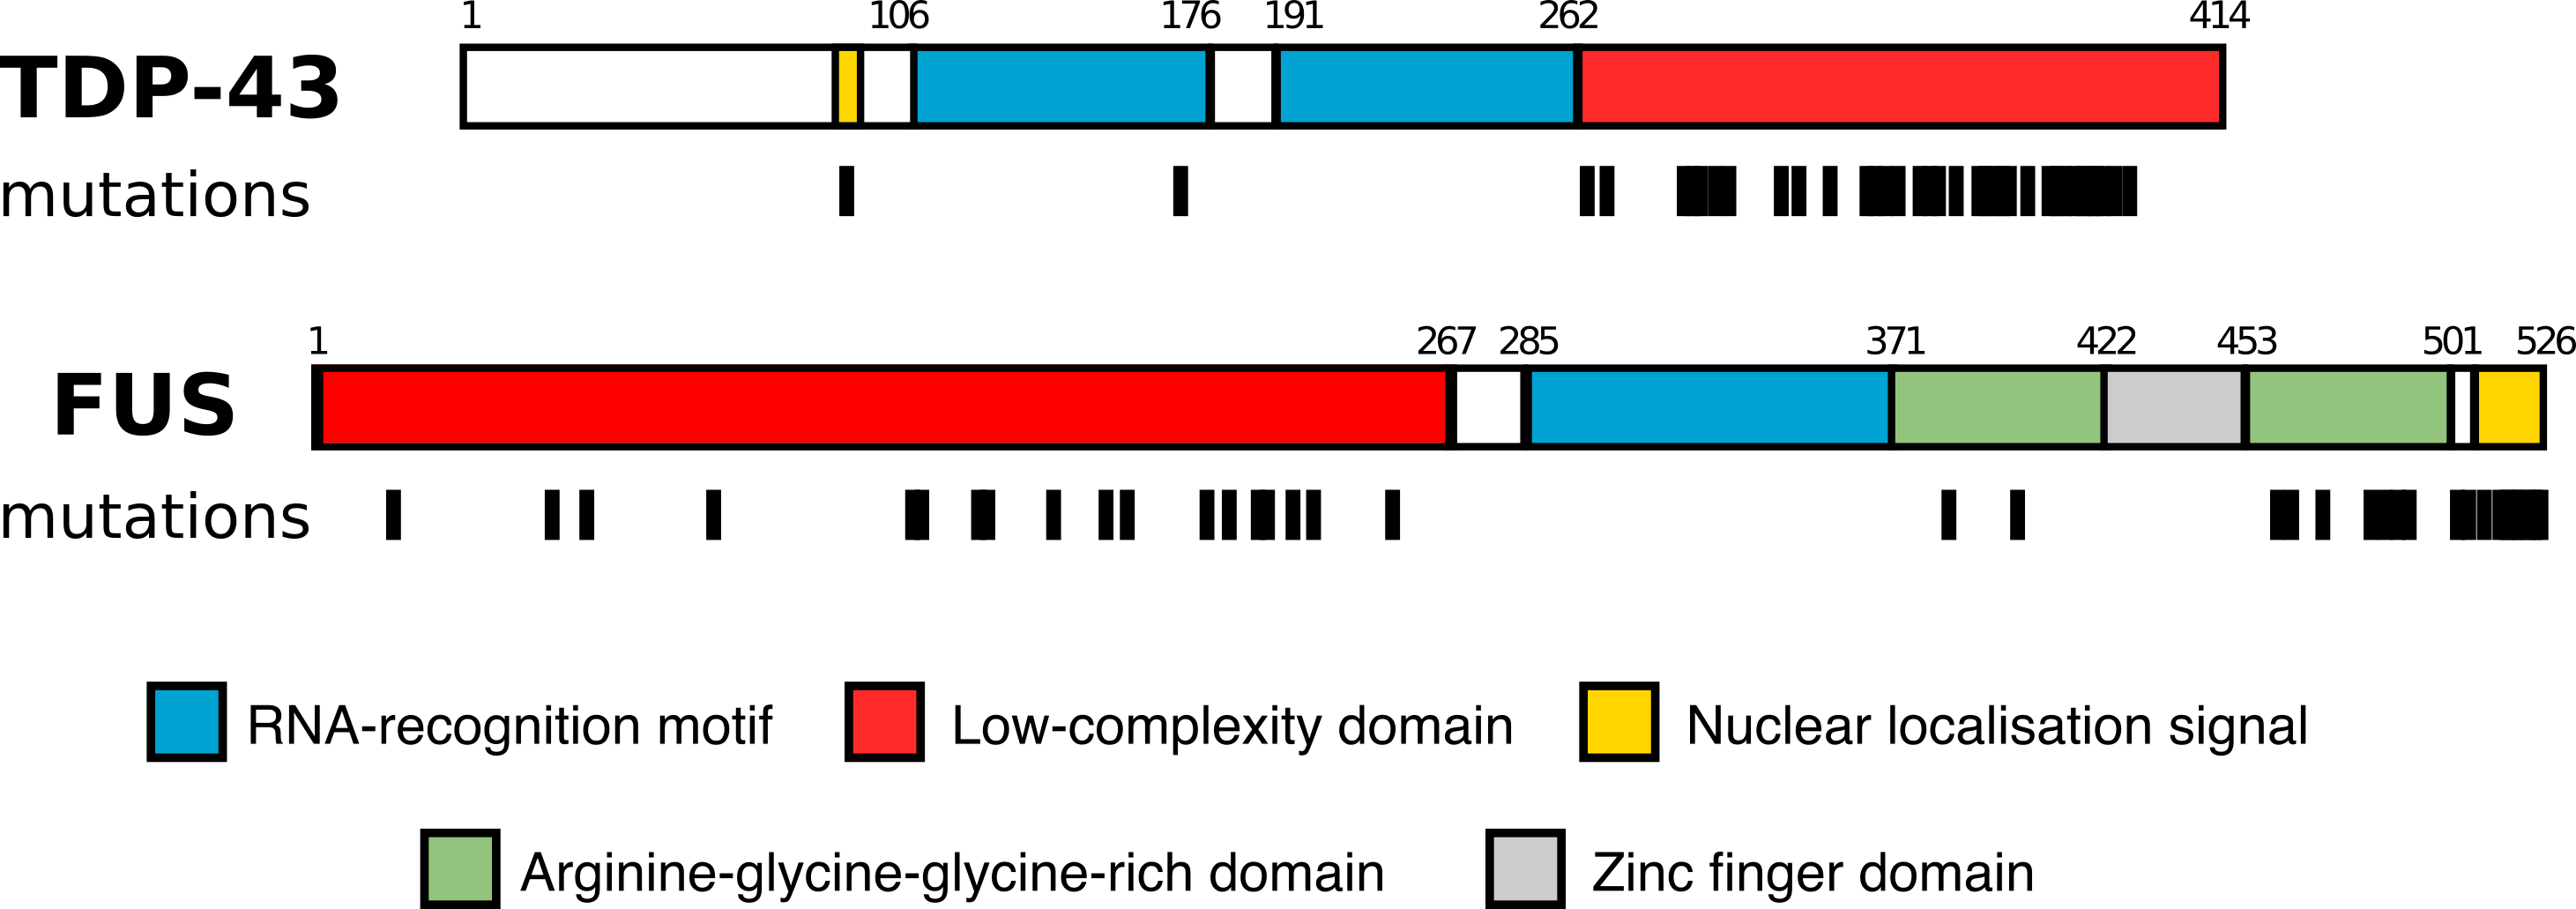
\includegraphics[width=\textwidth]{Figures/01_introduction/tdp_fus_structures.png}
	\caption[Protein domains of TDP-43 and FUS]{
		\textbf{Protein domains of TDP-43 and FUS}. Structures of the two proteins, coloured by functional domain. Positions of each mutation are represented by black bars. Figure adapted from \citep{Kapeli2017}. 
	}
	\label{fig:intro_domains}
\end{figure}


\subsection{TDP-43}

% intro
Transactive response DNA-binding protein 43 kDa (TDP-43) is a ubiquitously expressed RNA and DNA-binding protein encoded by the \emph{TARDBP} gene. 
It contains two RNA-recognition motifs, a nuclear localisation signal and a long glycine-rich low-complexity domain (Fig \ref{fig:intro_domains}).
Loss of TDP-43 from the nucleus accompanied by TDP-43 positive inclusions in the cytoplasm of cortical and spinal cord neurons is the hallmark pathology found in nearly all sporadic cases of ALS as well as the majority of non-Tau cases of FTD \citep{Neumann2006,Arai2006} as well as cases of Alzheimer's disease \citep{LaClair2016} and Huntington's Disease \citep{Doi2008}. 
Cytosolic TDP-43 has also been found in mouse models of traumatic brain injury, suggesting mislocalisation is a general neuronal stress response \citep{Moisse2009}. 
In addition, missense mutations in \emph{TARDBP} have been shown to cause familial ALS \citep{Sreedharan2008-xv}.  Mutations cluster in the low-complexity domain \citep{Kapeli2017};(Fig. \ref{fig:intro_domains}).
These findings point to a key role of TDP-43 in the development of ALS/FTD. 
There is still much debate on whether the mislocalisation of TDP-43 plays a role in neurodegeneration through a loss of normal nuclear function or a gain of cytoplasmic function.  
A further question is the influence of rare mutations in the TDP-43 low-complexity domain and how they contribute to pathology.

\subsubsection{Roles in RNA regulation}

TDP-43 is a predominantly nuclear protein but can shuttle to the cytoplasm \citep{Ayala2008}. 
This has implicated it both in nuclear roles in transcription and splicing, but also in RNA transport and translation. 
In splicing, TDP-43 binds UG-rich RNA motifs \citep{Buratti2001a, Buratti2001}, validated by X-ray crystallography \citep{Lukavsky2013}. 
TDP-43 binding can either repress or enhance cassette exon splicing depending on the motif position, as was found for individual genes \citep{Mercado2005-js,Bose2008-du,Shiga2012-it}.
This was expanded genome-wide by RNA-protein interaction experiments to find RNA targets of TDP-43 and correlate TDP-43 binding with cassette exon splicing \citep{Polymenidou2011,Tollervey2011,Kapeli2016}. % RNA maps?
For cassette exons, TDP-43 binds on top of or close to exons which it represses and further away from the exons it enhances \citep{Tollervey2011}, similarly to NOVA proteins.
However, the majority of TDP-43 binding was found to be deep within introns and on 3\'\ untranslated regions (3\'\ UTRs).
Long intron genes were strongly downregulated under TDP-43 depletion \citep{Polymenidou2011}, suggesting an important role for TDP-43 in their splicing and stabilisation. 
TDP-43 knockdown was found to cause the emergence of a set of cryptic exons from poorly conserved introns \citep{Ling2015}, suggesting that intronic binding of TDP-43 acts to repress cryptic splice sites. 
Unlike hnRNP C this has not been linked to a particular class of retrotransposon element, despite TDP-43 being observed to bind a range of retrotransposons including Alu elements \citep{Li2012,Zarnack2013,Kelley2014}.
Attempts to correlate TDP-43's effect on the splicing of a gene with a change in the level of the subsequent protein have found few examples \citep{DeConti2015,Stalekar2015}.

In the cytoplasm TDP-43 binds a set of genes at the 3\'\ UTR \citep{Colombrita2012} and can form cytoplasmic RNA granules which in neurons are transported along axons \citep{Alami2013, Fallini2012}. This gives TDP-43 a role in local translation.
TDP-43 has been shown to either repress or enhance the translation of a small number of target transcripts \citep{Majumder2012, Majumder2016, Neelagandan2018}.
In addition, many of the proteins identified to interact with TDP-43 are involved in translation \citep{Freibaum2010-hw}.
TDP-43 controls its own translation by autoregulation.
This is achieved by TDP-43 binding the 3\'\ UTR of the \textit{TARDBP} transcript \citep{Ayala2011,Koyama2016}. 
Under conditions of cellular stress, translation is temporarily paused when actively translated mRNAs and RNA-binding proteins assemble into processing bodies and stress granules \citep{Anderson2008}. 
This assembly relies on protein-protein interactions between low-complexity domains of RNA-binding proteins.
TDP-43 is recruited to stress granules \citep{Colombrita2009} and ALS-linked mutations in the low-complexity domain increase this level of recruitment \citep{Liu-Yesucevitz2010}.
These granules can then rapidly disassemble once stress is stopped.

% other roles for TDP in RNA
%Other roles in RNA regulation have been observed for TDP-43, such as microRNA creation \citep{Kawahara2012} and the binding of retrotransposon elements 

\subsubsection{Roles in disease}

In affected neurons and glial cells with ALS/FTD, TDP-43 leaves the nucleus and forms protein aggregates in the cytoplasm \citep{Neumann2006}. 
Efforts in understanding TDP-43 in disease have looked at both loss and gain- of function, as well as the relevance of TDP-43 mutations to pathogenesis.

% TDP aggregates
TDP-43 aggregates contain fragments of the TDP-43 C-terminal as well as full length TDP-43 that are phosphorylated and ubiquitinated \citep{Neumann2006,Arai2006, Bosque2013, Hasegawa2008}.
These aggregates are toxic to neurons  \citep{Zhang2009} and also contain a number of other RNA-binding proteins \citep{Dammer2012}.
TDP-43 can spontaneously aggregate with itself, and mutations in the low complexity domain increase the propensity to do so \citep{Johnson2009}.
TDP-43 aggregates are types of amyloid \citep{Fang2014}, specific structures that are toxic to neurons and found in multiple neurodegenerative diseases.
The relationship between the dynamic role of TDP-43 in RNA granules, including stress granules, and the formation of toxic TDP-43 aggregates is not yet fully understood.

Global loss of TDP-43 is lethal in the mouse embryo \citep{Kraemer2010} and postnatal deletion leads to rapid death \citep{Chiang2010}. 
Conditional knockout of TDP-43 in mouse postnatal motor neurons causes a gradual degeneration of affected neurons and atrophy of muscle \citep{Iguchi2013}. 

Overexpression of wildtype human TDP-43 in mice caused motor neuron degeneration in the spinal cord and severe motor impairment in proportion to the dose of the transgene \citep{Wils2010, Shan2010}.
However toxicity caused by TDP-43 overexpression occurs in mice without the observation of TDP-43 aggregates \citep{Wegorzewska2009, Barmada2010}.
Conversely, wildtype human TDP-43 was not found to be toxic when expressed at a physiological level \citep{Arnold2013} and only the ALS-causing mutant forms were found to cause motor neuron degeneration. 
Again, this occurred without observed TDP-43 loss in the nucleus nor cytoplasmic aggregation. 
This works suggests that TDP-43 toxicity to neurons does not require TDP-43 aggregates to form.
Clearly neurons are very sensitive to the expression level of TDP-43 protein, and this is compounded by autoregulation. 
Therefore, any changes in TDP-43 protein levels through knockdown or over-expression will interfere with this feedback loop, making it hard to gauge the true expression change of a particular targeting strategy. 





%% what do I do about FUS here?
%Rare ALS-causing mutations have been found in another RNA-binding protein, FUS \citep{Vance2009-ye}, further raising the possibility that the impairment of RNA processing is a central cause of ALS.  TDP-43 and FUS have both been shown to bind a set of overlapping RNA targets \citep{Lagier-Tourenne2012-wa}.

%%TDP-43 and splicing
%%FIRST thing to be found on TDP-43. How much agreement between studies?

%"TDP-43 binds to (GU)16 repeats in apoA-II intron 2 and represses exon 3 splicing" \citep{Mercado2005}

%965 altered splicing events seen in adult mouse brain with TDP-43 depletion \citep{Polymenidou2011}
%%\citep{Tollervey2011} TDP-43 can bind within exons to repress them but can also bind up or downstream of them. Generally binding further away (up to 250nt from the exon) acts to enhance inclusion.
%
%Other splicing factors are perturbed in TDP-FTD \citep{Mohagheghi2015}: "the expression of hnRNPA1/A2 and PTB/nPTB is significantly altered in patients with frontotemporal dementiawith TDP-43-positive inclusions" A large number of splicing factors also alter the inclusion of SORT1 exon 17b.


%tDP-43 and POLDIP3 splicing - annotated exon 3 in POLDIP is enhanced by TDP, loss of TDP reduces the inclusion. Laser capture of neurons from ALS brain show a reduction in exon 3 containing POLDIP3. POLDIP3 involved in maintaining cell size. Exon3 lacking POLDIP3 cannot rescue cell size as well from POLDIP3 or TDP-43 knockdown. \citep{Shiga2012}.

%"Validation of the bona fide splicing events that are consistent data, both in neuronal and non-neuronal cell lines demonstrated that TDP-43 substantially alters the levels of isoform expression" in four genes but only in 2 these changes could also be confirmed at the protein level \citep{DeConti2015}. - Assessing splicing changes is hard and there is no guarantee that this leads to changes in protein level. 

%Repeat elements - dpn't put in introuction
%5




%%HERE is a bunch of different findings from TDP-43 animal models
%How does each support loss- or gain-of-function hypothesis?

%"knockout of transactive response DNA-binding protein 43 in mouse postnatal motor neurons using Cre/loxp system, progressive weight loss and motor impairment around the age of 60 weeks, and exhibited degeneration of large motor axon, grouped atrophy of the skeletal muscle, and denervation in the neuromuscular junction. The spinal motor neurons lacking transactive response DNA-binding protein 43 were not affected for 1 year, but exhibited atrophy at the age of 100 weeks; whereas, extraocular motor neurons, that are essentially resistant in amyotrophic lateral sclerosis, remained preserved even at the age of 100 weeks" \citep{Iguchi2013}

%"increased excitatory synaptic inputs and dendritic spine densities in early presymptomatic mice carrying a TDP-43Q331K mutation" \citep{Fogarty2016}

%"postnatal deletion of Tardbp in mice caused dramatic loss of body fat followed by rapid death. Moreover, conditional Tardbp-KO ES cells failed to proliferate" \citep{Chiang2010}

%"mice expressing a mutant frm of human TDP-43 develop a progressive and fatal neurode- generative disease reminiscent of both ALS and FTLD-U. Despite universal transgene expression throughout the nervous system, pathologic aggregates of ubiquitinated proteins accumulate only in specific neuronal populatioons, including layer 5 pyramidal neu- rons in frontal cortex, as well as spinal motor neurons, recapitu- lating the phenomenon of selective vulnerability seen in patients with FTLD-U and ALS. Surprisingly, cytoplasmic TDP-43 aggregates are not present, and hence are not required for TDP-43-induced neurodegeneration." \citep{Wegorzewska2009} Overexpression of mutant human TDP A315T in mice at levels "3-fold higher" 

%"Mice expressing hu- man TDP-43 in neurons exhibited growth retardation and prema- ture death that are characterized by abnormal intranuclear inclusions composed of TDP-43 and fused in sarcoma/translocated in liposarcoma (FUS/TLS), and massive accumulation of mitochon- dria in TDP-43-negative cytoplasmic inclusions in motor neurons, lack of mitochondria in motor axon terminals, and immature neuromuscular junctions" \citep{Shan2010} 

%\citep{Igaz2011} "Expression of either hTDP-43-ΔNLS or hTDP-43-WT led to neuron loss in selectively vulnerable forebrain regions, corticospinal tract degeneration, and motor spasticity recapit- ulating key aspects of FTLD and primary lateral sclerosis. Only rare cytoplasmic phosphorylated and ubiqui- tinated TDP-43 inclusions were seen in hTDP-43-ΔNLS mice"

%"Two ALS-causing mutants (TDP-43Q331K and TDP-43M337V), but not wild-type human TDP-43, are shown here to provoke age-dependent, mutant-de- pendent, progressive motor axon degeneration and motor neu- ron death when expressed in mice at levels and in a cell type- selective pattern similar to endogenous TDP-43. Mutant TDP-43-dependent degeneration of lower motor neurons occurs without: (i) loss of TDP-43 from the corresponding nuclei, (ii) accumulation of TDP-43 aggregates, and (iii) accumulation of insoluble TDP-4" \citep{Arnold2013}




%tTDP-43 regulates the levels of other neurodegenerative disease mRNAs like FUS and PGRN \citep{Polymenidou2011} and preferentially stabilises the expression of long intron genes, something shared with FUS. iCLIP of TDP-43 showed "unusually long clusters of TDP-43 binding at deep intronic positions downstream of silenced exons." \citep{Tollervey2011}.

%tTDP-43 and UG motifs: "TDP-43 has a unique capacity to recognize dispersed clusters of UG-rich motifs, or to spread its RNA binding to positions proximal to the UG-rich motifs" \citep{Tollervey2011} Both RRMs come together to bind UG-rich RNA \citep{Lukavsky2013} - interactions between the two RRMs are crucial for RNA binding




%%OTHER stuff TDP does


%%RNA transport
%\citep{Alami2013} finds "TDP-43 is a component of mRNP transport granules in neurons, including human stem cell-derived motor neurons, and identify a new role for TDP-43 in the cytoplasm supporting anterograde axonal transport of target mRNAs from the soma to distal axonal compartments"

%%TDP-43 autoregulation 
%first seen by Polymenidou \citep{Polymenidou2011} then assessed by \citep{Ayala2011} \citep{Er??ndiraAvenda??o-V??zquez2012} and \citep{Koyama2016}. TDP-43 binds the 3'UTR of the TARDBP mRNA to prevent the usage of the proximal polyA site. The longer TARDBP 3'UTR transcript undergoes multiple splicing rounds that ultimately reduce the levels of TDP-43 protein. With TDP-43 depletion the proximal polyA site is used and the levels of cytoplasmic TARDBP mRNA are increased.

%%TDP-43 proteomics
%proteomic study on loss of TDP-43 \citep{Stalekar2015} "TDP-43 is an important regulator of RNA metabolism and intracellular transport."
%%TDP interactome \citep{Freibaum2010-hw} shows TDP-43 interacts with multiple splicing factors (MATR3/hnRNPAB/SFPQ) as well as ribosomal proteins. "Disease-causing mutations in TDP- 43 (A315T and M337V) do not alter its interaction profile. TDP-43 interacting proteins largely cluster into two distinct interaction networks, a nuclear/splicing cluster and a cytoplasmic/translation cluster, strongly suggesting that TDP-43 has multiple roles in RNA metabolism and functions in both the nucleus and the cytoplasm"

%Impaired nuclear import of WT TDP-43 as general mechanism
%Screen of 82 nuclear import proteins "knockdowns of karyopherin-b1 and cellular apoptosis susceptibility protein resulted in marked cyto- plasmic accumulation of TDP-43." \citep{Nishimura2010} "considerable reduction in expression of cellular apoptosis susceptibility protein in frontotemporal lobar degeneration."




%Prion-like C terminal 
%
%"TDP-43 does have inter-domain in- teractions which is coordinated by the intrinsically-disordered prion-like domain" \citep{Wei2016}
%
%Mitochondria
%%TDP-43 localises to the mitochondria of motor neurons and this increases with the increase in cytoplasmic TDP in ALS. TDP-43 mutations increase mitochondrial localisation. In mitochondria TDP binds complex I components TDP-43 protein sequence contains multiple mitochondrial import sequences. Competitive inhibition of TDP-43's mitochondrial localisation rescues neurotoxicity. \citep{Wang2016}
%
%
%%TDP depletion in Alzheimers - "TDP-43 proteinopathy, initially associated with ALS and FTD, is also found in 30–60\% of Alzheimer’s disease (AD) cases and correlates with worsened cognition and neurodegeneration." Some forebrain AD sensitive neurons are selectively vulnerable to TDP-43 loss.
%




% FUS


\subsection{FUS}

Fused in sarcoma is a ubiquitously expressed RNA-binding protein encoded by the \textit{FUS} gene. 
The FUS protein consists of a long low-complexity domain, an RNA-recognition motif, two arginine-glycine-glycine domains, a zinc finger domain and a N-terminal nuclear localisation signal (Fig. \ref{fig:intro_domains}).
%The previously identified nuclear export signal is in fact non-functional and FUS leaves the nucleus through passive diffusion \citep{Ederle2018}. 
FUS is a member of the FET family of RNA binding proteins, sharing high sequence homology with EWSR1 and TAF15 \citep{Kovar2011}.
Mutations in \textit{EWSR1} and \textit{TAF15} have both been found in a small number of ALS patients \citep{Neumann2011, Couthouis2011,Ticozzi2011,Couthouis2012}.
Over 40 mutations in FUS have been found to cause ALS, accounting for around 5\% of familial cases and 1\% of sporadic cases \citep{Vance2009-ye,Kwiatkowski2009}.  
Mutations cluster in the low complexity domain and the nuclear localisation signal.
FUS-ALS is distinguished from sporadic ALS by its aggressive early onset and the presence of FUS protein in cytoplasmic aggregates and not TDP-43. 
FUS mutations have also been found in a very small number of FTD cases \citep{VanLangenhove2010,Broustal2010}.
However, FUS-positive inclusions are seen in around 10\% of FTD cases in the absence of any FUS mutation \citep{Neumann2009}. 
Additionally, FUS has also been detected in aggregates from cell and mouse models of Huntington's disease \citep{Doi2008, Kino2016}.

\subsubsection{Roles in RNA regulation}

Although predominantly localised to the nucleus, FUS appears have a role in every step of RNA processing in both the nucleus and cytoplasm. 
As a splicing factor it binds to GGU motifs within introns and 3\'\ UTR sequences to either enhance or repress exon inclusion and polyadenylation \citep{Rogelj2012,Lagier-Tourenne2012}.
As with TDP-43, FUS preferentially binds within introns and 3\'\ UTRs \citep{Lagier-Tourenne2012,Rogelj2012,Ishigaki2012}. 
However the overlap between FUS and TDP-43 RNA targets is small  \citep{Lagier-Tourenne2012,Rogelj2012,Colombrita2012, Honda2014}.
A small number of genes were found to have FUS binding antisense to the promoter \citep{Ishigaki2012}.
In genes with long (>100kb) introns, FUS binding has a sawtooth pattern which appears to decline over the length of the intron \citep{Rogelj2012}. 
FUS depletion leads to downregulation of long intron genes \citep{Lagier-Tourenne2012}, suggesting FUS plays a role in stabilising the splicing of particularly long introns.
FUS also has a role in polyadenylation through its interaction with RNA polymerase II \citep{Schwartz2012} as it can stall transcription at 3\'\ UTRs to encourage premature polyadenylation \citep{Masuda2015}. 
FUS has been observed to modulate 3\'\ end processing of RNA, as observed in the GluA1 AMPA receptor subunit \citep{Udagawa2015}. % what does it modulate?
FUS knockdown has also been shown to alter levels of intron retention, particularly in splicing factors \citep{VanBlitterswijk2013, Nakaya2013}.

In transcription, FUS interacts with RNA polymerase II, which could modulate transcription elongation speed \citep{Schwartz2012}.
FUS interacts with both the major spliceosome via the U1 snRNP \citep{Sun2015a, Yu2015a} and the minor spliceosome through binding to  the U11 snRNP \citep{Reber2016}, both of which define the 5\'\ splice site at major or minor introns.
Within splicing factor networks FUS also interacts with TDP-43, MATRIN3, hnRNP A1, PTBP1 and other SR splicing factors \citep{Lagier-Tourenne2012,Yamaguchi2016,Yang1998,Meissner2003, Kamelgarn2016}. 
Some of these interactions are RNA-dependent \citep{Kamelgarn2016}.
The role of FUS in splicing is therefore highly complex and nuanced.

Beyond mRNA, FUS facilitates the creation of both microRNA \citep{Morlando2012} and circular RNA \citep{Errichelli2017}, two RNA species with complex regulatory functions.
In the cytoplasm FUS has also been observed in RNA transport granules \citep{Kanai2004, Fujii2005}.
FUS is also present in cytoplasmic SMN complexes which create the spliceosomal snRNP complexes  \citep{Yamazaki2012,Groen2013}.
% Stress granules
As with TDP-43, FUS aggregation has been linked to stress granule formation.
FUS itself is recruited into stress granules \citep{Andersson2008,Yasuda2013}. 
NLS mutations increase cytoplasmic FUS and increase FUS stress granule recruitment \citep{Dormann2010, Bosco2010}.
This requires RNA-binding activity of FUS to occur \citep{Daigle2013}	.
FUS aggregates found in ALS/FTD patients also contain stress granule proteins \citep{Dormann2010} suggesting a link between stress granule formation and disease.
Like TDP-43, FUS can control its own translation by autoregulation.
This is thought to occur by FUS binding creating an NMD-sensitive exon skipping isoform \citep{Zhou2013}.



\subsubsection{Roles in disease}

Although causative ALS mutations have been found throughout the FUS protein, mutations associated with the lowest age of onset and shortest disease course are clustered in the proline-tyrosine) nuclear localisation signal (NLS). 
Nuclear import of FUS is controlled by the nuclear import receptor protein transportin binding to the NLS \citep{Dormann2010}.
The most aggressive FUS mutations either mutate the key proline residue in the terminal PY motif (P252L; \citep{Chio2009}) or remove the NLS entirely through a frameshift (G466VfsX14; \citep{DeJesus-Hernandez2010}) or a stop codon (R495X; \citep{Bosco2010}). 
Patients with these NLS ablating mutations tend to die in their early 20s whereas patients with NLS mutations further from the PY sequence have disease onsets resembling sporadic ALS \citep{Shang2016}.
The fact that NLS removal causes such an aggressive form of the disease suggests that mislocalisation of FUS in the cytoplasm is the key pathogenic event. However, whether this is due to a loss of nuclear FUS or toxic gain of function from the increased cytoplasmic FUS is still unclear.
Like TDP-43, FUS protein can spontaneously aggregate \textit{in vitro} through its low complexity domain \citep{Murray2017}. 
NLS mutations do not alter the propensity of FUS to self-aggregate \citep{Sun2011}.
Instead NLS mutations mislocalise FUS to the cytoplasm, which may encourage aggregation. The interaction between transportin and the FUS NLS has recently been recognised to promote the dissolution of FUS aggregates \citep{Guo2018, Yoshizawa2018}. 
Reduced nuclear FUS would also impair autoregulation, increasing translation of FUS protein. This would then increase cytoplasmic FUS.
% animal models
In the mouse, complete knockout of endogenous FUS is lethal in an inbred C57BL/6 J background  \citep{Hicks2000, Kuroda2000} but survive until adulthood on a mixed background with no apparent motor deficits at 90 weeks of ages \citep{Kino2015}.
% overexpression
Overexpression studies have found a dosage dependence for the expression of human FUS to cause disease symptoms \citep{Verbeeck2012,Mitchell2013, Shiihashi2016}, with neurodegeneration and death only seen when human mutant FUS was highly expressed.
Overexpression of NLS mutant FUS does not appear to alter the splicing of FUS RNA targets \citep{Shiihashi2016}, despite mutant FUS interacting with the endogenous wildtype FUS \citep{Qiu2014}.
% gain of function
Other studies suggest a gain of function mediated by mutant FUS being responsible for neurodegeneration. 
Post-natal knockout of endogenous FUS  in motor neurons did not lead to motor dysfunction \citep{Sharma2016}.
A direct comparison between FUS knockout and mutation demonstrated embryonic lethality in both conditions, but with motor neuron loss only seen in the mutant mice \citep{Scekic-zahirovic2016}.  
There are still no mouse models of FUS ALS that study mutant FUS at a physiological expression level.



%of human FUS in mice causes a progressive motor neuron loss and death by 3 months, accompanied by cytoplasmic FUS protein expression \citep{Mitchell2013}. 
%This occured only when the FUS knockout transgene was homozygous, suggesting a dose sensitivity to the wildtype human protein for neurodegeneration. 
%
%Expression of mutant human FUS in the mouse brain caused an increased cytoplasmic accumulation of FUS relative to that of the wildtype, though no neurodegeneration was observed after 3months \citep{Verbeeck2012}. 
%
%Verbeeck and colleagues generated mice overexpressing FUS with either wildtype, an NLS mutation (R521C) or the NLS-ablating $\Delta14$ mutation \cite{Verbeeck2012}. Only mutant FUS was found to localise to the cytoplasm and the $\Delta14$ mutation also showed formation of cytoplasmic aggregates. 
%Overexpressing NLS-ablated FUS in mice leads to motor deficits and neuronal loss in motor cortex \citep{Shiihashi2016}. The authors did not observe any changes in FUS-mediated splicing activity.
%
%Overexpression of human FUS causes a progressive motor neuron loss and death by 3 months, accompanied by cytoplasmic FUS protein expression \citep{Mitchell2013}. 
%This only occurred when the FUS transgene was homozygous, suggesting a dose sensitivity to the wildtype human protein for neurodegeneration. 
%
%Qiu and colleagues created a transgenic mouse overexpressing R521C mutant FUS \citeyear{Qiu2014}. 
%They found that mutant FUS interacted with endogenous wildtype FUS and wildtype FUS protein is increased in the presence of mutant FUS. They also found neurodegeneration and DNA damage phenotypes, as well as widespread intron retention changes. 
%
%
%



\section{Aims of my PhD} 

% TDP and FUS biology - what do they do?

% TDP and FUS mouse models - how to better understand disease

Understanding the role of TDP-43 and FUS in disease requires studying their roles in neuronal cells.
The aim of my PhD is to capitalise on the RNA-seq revolution and bring together disparate datasets to assess the nature of RNA regulation by TDP-43 and FUS.
I then apply that insight to novel animal models of disease generated by the UCL Institute of Neurology.


\section{Overview of chapters}

\subsection{Cryptic splicing occurs in published TDP-43 but not FUS depletion data}
TDP-43 has been observed to repress non-conserved intronic sequence from recognition by the spliceosome \citep{Ling2015}. 
I combined multiple public datasets on TDP-43 or FUS depletion and developed a method to discover and quantify cryptic splicing.
I expanded the number of cryptic exons found to be repressed by TDP-43. 
Conversely I did not find evidence of cryptic exon splicing in FUS knockdown in human and mouse cells.

\subsection{FUS mutant mice show progressive changes in mitochondrial and ribosomal transcripts}
Most attempts to model FUS ALS in mice either knock out endogenous FUS or over-express human mutant forms of FUS. 
Any study of RNA processing and/or motor neuron toxicity in these models is therefore confounded.
Dr Anny Devoy developed a new mouse model where an aggressive ALS mutation was knocked in to endogenous mouse FUS. 
This allows for the study of mutant FUS when expressed at a physiological level. 
I analysed RNA-seq data collected from two tissues and time points and observed a progressive change in mitochondrial and ribosomal transcripts restricted to the spinal cord.

\subsection{Loss and gain of TDP-43 splicing function in two mutant mouse lines}
ALS mutations in TDP-43 cluster in the C-terminal low-complexity region of the protein.
I studied RNA-seq datasets from two mutant mouse lines generated by random mutagenesis. 
One line had a mutation in the RNA-recognition motif which reduced the RNA-binding ability of TDP-43.
This was accompanied by cryptic exons, a sign of a loss of splicing function.
The second line had a mutation in the low-complexity domain.
I observed widespread skipping of normally constitutive exons, the inverse phenomenon to cryptic exon repression.

\subsection{ALS-causative FUS mutations impair FUS autoregulation through intron retention}
The most aggressive forms of ALS arise from mutations in the nuclear localisation signal of FUS.
I combined 3 embryonic mouse datasets where FUS was either knocked out or the nuclear localisation signal was removed.
This allowed me to jointly model the effects of the two different conditions, increasing detection power and confidence.
I observed substantial overlap in both gene expression and splicing, suggesting that the FUS mutations primarily reduce the nuclear function of FUS.
I identified a novel mechanism by which FUS could regulate its own translation.



% explain what RBPs do
% use examples from FUS and TDP-43 literature

% transcription

% splicing


% RNA transport

% Stress granules


%
%Introduce the two diseases. Introduce the RNA regulation theory of disease but also discuss the other possibilities

%Two bad neurodegenerative diseases
%Describe clinical presentations of both
%The ALS/FTD spectrum - linked through TDP-43 and FUS
%
%Evidence for RNA processing involvement in ALS/FTD
%
%
%%ALS/FTD and RNA-binding proteins


%In the case of TDP. FUS, A1/A2, Matr3, RBPs are mutated but with C9 RBPs are sequestered by the repeat. And yet all patients have similar phenotype.


% the biological problem
% from the paper:
%explain RNA regulation
%
%What do neurons need?
%Long genes with complex isoforms to increase protein diversity
%Need to transport RNA and protein over long distnace
%Local translation at synapses - control over protein expression


% progress in animal models of disease - put in discussion?
%The field as a whole is progressing towards more subtle and genuinely disease-like models; from the first knock-out mice, to over-expression of human mutant proteins to the more modern knock-in models where the mutant protein is expressed at a physiological level. While we can be more confident that the results from these more sophisticated experiments are closer to the the truth in humans, they suffer from a much longer generation time due to replicating diseases of old age. Changes in RNA may be subtler than we currently have the power to detect or more baroque than we can yet understand. 


% review of FUS functions citep{Ling2013}

%%FUS proteinopathies - citation?


%%TAF15 and EWSR1 share prion like domains with TDP-43 and FUS, missense variants in TAF15 in ALS patients \citep{Couthouis2011}
%%EWSR1 and TAF15 also in FTD-FUS cytoplasmic inclusions \citep{Neumann2011}
%variants in EWSR1 in ALS \citep{Couthouis2012}
%rare variants found in TAF15 in fALS causes \citep{Ticozzi2011-bs}


%Recent studies have demonstrated an interaction with RNA-polymerase II and the U1 snRNP \citep{Yu2015,Sun2015a}. 
%%SMN:
%"Expression of different FUS mutants (R521C, R521H, P525L) in neurons caused axonal defects. A protein interaction screen performed to explain these phenotypes identified numerous FUS interactors including the spinal muscular atrophy (SMA) causing protein survival motor neuron (SMN). Biochemical experiments showed that FUS and SMN interact directly and endogenously, and that this interaction can be regulated by FUS mutations" \citep{Groen2013}.
%"This studyshows that neuronal aggre- gatesformedbymutantFUSproteinmayaberrantlysequesterSMNandconcomitantlycauseareductionofSMN levels in the axon, leading toaxonal defects"
%
%It has also been linked to the minor splicesome \citep{Reber2016}. 
%
%Other roles for FUS:
%binding RNA polymerase II \citep{Schwartz2012}
%chromatin binding through binding to SAF3B and MATR3 \citep{Yamaguchi2016}
%regulates the expression of other RNA-binding proteins \citep{Nakaya2013}
%\citep{Rogelj2012}: binds GGU motifs within introns - less strongly than TDP-43 binds UG, represses inclusion of cassette exons, regulates splicing of Ewsr1 - same protein family as FUS. Genes with FUS-regulated splicing are enriched for neuronal development
%alternate polyadenylation \citep{Masuda2015} - position specific -  stalls RNA Polymerase II to initiate alternate polyadenylation of shorter transcripts
%
%Stress granules:
%	mutant FUS, but not wildtype FUS, forms stress granules in response to stress in Zebrafish \citep{Bosco2010}
%	"RNA-binding-deficient FUS strongly localized to the nucleus of Drosophila motor neurons and mammalian neuronal cells, whereas FUS carrying ALS-linked mutations was distributed to the nucleus and cytoplasm. Importantly, we determined that incorporation of mutant FUS into the SG com- partment is dependent on the RNA-binding ability of FUS" \citep{Daigle2013}
%
%\citep{Yasuda2013}: FUS recruited to APC-dependent granules which are translationally active, unlike stress granules. FUS promotes translation within these granules 
%
%Autoregulation:
%	\citep{Zhou2013} FUS binds its own introns to regulate its own expression - mutant FUS leaves the nucleus so cannot reduce its own expression levels - feedback. 
